\documentclass[12pt]{article}
\usepackage{graphicx}
\usepackage{enumerate}
\usepackage{amsmath}

\setlength{\oddsidemargin}{.1in}
\setlength{\textwidth}{6.3in}
\setlength{\textheight}{8.9in}
\setlength{\topmargin}{-.5in}

\title{Numerically simulating the dynamics of the pendulum and cart}
\date{}

\begin{document}

\maketitle

\section{Kinematics}

Consider a cart of mass $M$, motorized and free to move along the x-axis upon a frictionless track. A pendulum bob of mass $m$ is attached to the cart by a rigid, massless, freely swinging rod of length $l$. Let's start by writing down the kinematics---that is, the position, velocity, and acceleration---for each of the cart and bob.

For the cart,

\begin{align}
\mbox{position:} &\quad x \mathbf{\hat{x}} \nonumber\\[5pt]
\mbox{velocity:} &\quad x' \mathbf{\hat{x}} \nonumber\\[5pt]
\mbox{acceleration:} &\quad x'' \mathbf{\hat{x}}. \nonumber
\end{align}

And for the bob,

\begin{align}
\mbox{position:} &\quad (x + l \sin{\theta}) \mathbf{\hat{x}} + l \cos{\theta} \mathbf{\hat{y}} \nonumber\\[5pt]
\mbox{velocity:} &\quad (x' + l \theta' \cos{\theta}) \mathbf{\hat{x}} - l \theta' \sin{\theta} \mathbf{\hat{y}} \nonumber\\[5pt]
\mbox{acceleration:} &\quad (x'' + l \theta'' \cos{\theta} - l \theta'^2 \sin{\theta}) \mathbf{\hat{x}} - (l \theta'' \sin{\theta} + l \theta'^2 \cos{\theta}) \mathbf{\hat{y}}. \nonumber
\end{align}

\section{Forces}

We can list the forces acting on each of the cart and bob as well (see Fig. \ref{fig:free_body}).

\begin{figure}
\center
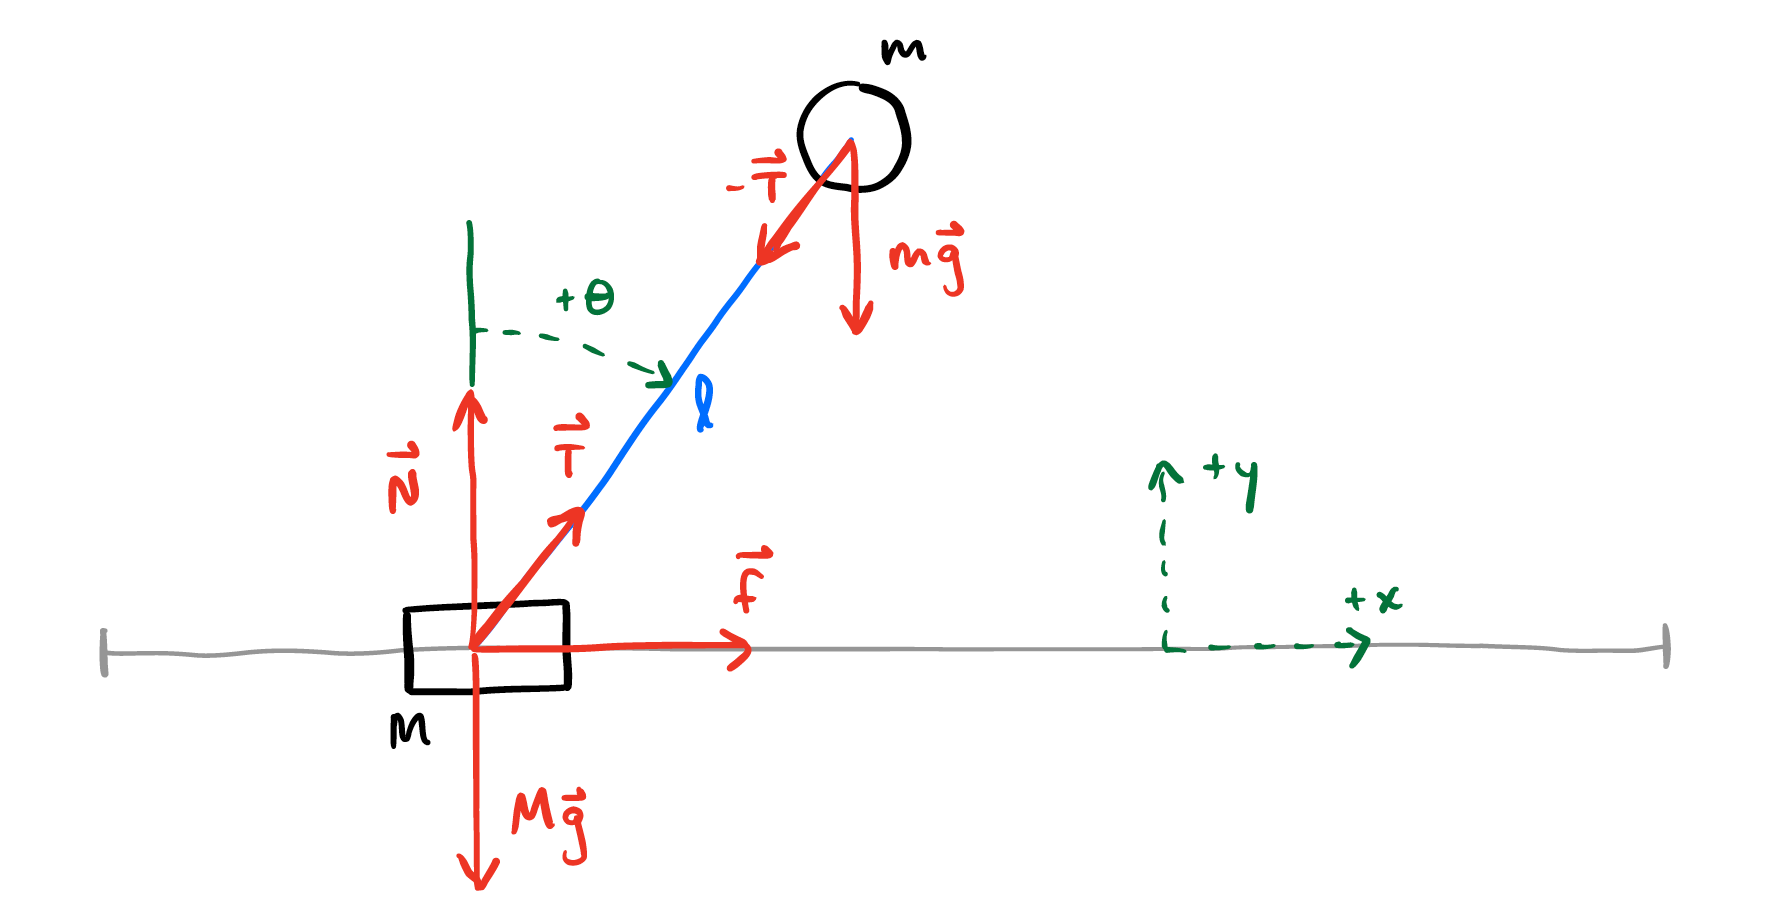
\includegraphics[width=0.9\linewidth]{free_body.png}
\caption{Free body diagram for our setting of the cart and pendulum.}
\label{fig:free_body}
\end{figure}

The cart experiences

\begin{align}
\mbox{force due to gravity:} &\quad {-M} g \mathbf{\hat{y}} \nonumber\\[5pt]
\mbox{rod tension:} &\quad T \sin{\theta} \mathbf{\hat{x}} + T \cos{\theta} \mathbf{\hat{y}} \nonumber\\[5pt]
\mbox{normal force on track:} &\quad N \mathbf{\hat{y}} \nonumber\\[5pt]
\mbox{motor force:} &\quad f \mathbf{\hat{x}}. \nonumber
\end{align}

And the bob experiences

\begin{align}
\mbox{force due to gravity:} &\quad -m g \mathbf{\hat{y}} \nonumber\\[5pt]
\mbox{rod tension:} &\quad {-T} \sin{\theta} \mathbf{\hat{x}} - T \cos{\theta} \mathbf{\hat{y}}. \nonumber
\end{align}

\section{Equations of motion}

Using Newton's law $\mathbf{F_{net}} = m \mathbf{x''}$ to relate forces with kinematics, we get the two expressions which follow.

For the cart,

\begin{equation}
T \sin{\theta} \mathbf{\hat{x}} + f \mathbf{\hat{x}} - M g \mathbf{\hat{y}} + T \cos{\theta} \mathbf{\hat{y}} + N \mathbf{\hat{y}} = M x'' \mathbf{\hat{x}}.
\end{equation}

And for the bob,

\begin{equation}
-T \sin{\theta} \mathbf{\hat{x}} - m g \mathbf{\hat{y}} - T \cos{\theta} \mathbf{\hat{y}} = m x'' \mathbf{\hat{x}} + m l \theta'' \cos{\theta} \mathbf{\hat{x}} - m l \theta'^2 \sin{\theta} \mathbf{\hat{x}} - m l \theta'' \sin{\theta} \mathbf{\hat{y}} - m l \theta'^2 \cos{\theta} \mathbf{\hat{y}}.
\end{equation}

Separating these two equations into vector components gives four equations.

\begin{align}
\label{eq:a} \mbox{cart x:} &\quad T \sin{\theta} + f = M x'' \\[5pt]
\mbox{cart y:} &\quad {-M} g + T \cos{\theta} + N = 0 \\[5pt]
\label{eq:b} \mbox{bob x:} &\quad {-T} \sin{\theta} = m x'' + m l \theta'' \cos{\theta} - m l \theta'^2 \sin{\theta} \\[5pt]
\label{eq:c} \mbox{box y:} &\quad {-m} g - T \cos{\theta} = -m l \theta'' \sin{\theta} - m l \theta'^2 \cos{\theta}
\end{align}

Adding together equations (\ref{eq:a}) and (\ref{eq:b}) to eliminate $T$ gives

\begin{equation}
\label{eq:d} f = (M + m) x'' + m l \theta'' \cos{\theta} - m l \theta'^2 \sin{\theta}.
\end{equation}

Multiplying (\ref{eq:b}) through by $\cos{\theta}$ and multiplying (\ref{eq:c}) through by $-\sin{\theta}$ and then adding these together gives

\begin{equation}
\label{eq:e} m g \sin{\theta} = m x'' \cos{\theta} + m l \theta''.
\end{equation}

Our two equations of motion are (\ref{eq:d}) and (\ref{eq:e}). However, these must be rewritten to isolate $x''$ and $\theta''$ in each equation. This can be done algebraically or using \textit{Mathematica}, yielding

\begin{align}
x'' &= \frac{f + m l \theta'^2 \sin{\theta} - m g \sin{\theta} \cos{\theta}}{M - m - m \cos^2{\theta}} \\[5pt]
\theta'' &= \frac{-f \cos{\theta} + (M + m) g \sin{\theta} - m l \theta'^2 \sin{\theta} \cos{\theta}}{l (M + m - m \cos^2{\theta})}.
\end{align}

We can turn these two second-order ODEs into four first-order ODEs, yielding a form which will be suitable for numerical simulation via the Runge-Kutta method:

\begin{align}
x' &= v \\[5pt]
\theta' &= \omega \\[5pt]
v' &= \frac{f + m l \omega^2 \sin{\theta} - m g \sin{\theta} \cos{\theta}}{M + m - m \cos^2{\theta}} \\[5pt]
\omega' &= \frac{-f \cos{\theta} + (M + m) g \sin{\theta} - m l \omega^2 \sin{\theta} \cos{\theta}}{l (M + m - m \cos^2{\theta})}.
\end{align}

These are the equations of motion we will use for numerical simulation.

\section{Runge-Kutta update rule}
Now we will work out the update rules for simulating via the Runge-Kutta method. We can represent the system with a 5-dimensional state vector

\begin{align}
\mathbf{x} = (t, x, \theta, v, \omega) \in {\rm I\!R}^5, \quad \mbox{where, equivalently,} \\[5pt]
x_1 = t \nonumber\\[5pt]
x_2 = x \nonumber\\[5pt]
x_3 = \theta \nonumber\\[5pt]
x_4 = v \nonumber\\[5pt]
x_5 = \omega \nonumber.
\end{align}

So, our equations of motion become

\begin{align}
\frac{d}{dt} x_1 &= f_1(\mathbf{x}) = 1 \tag*{(passage of time; $dt = 1$)} \nonumber\\[5pt]
\frac{d}{dt} x_2 &= f_2(\mathbf{x}) = x_4 \tag*{(change in cart position; $\frac{dx}{dt} = v$)} \\[5pt]
\frac{d}{dt} x_3 &= f_3(\mathbf{x}) = x_5 \tag*{(change in pendulum angle; $\frac{d\theta}{dt} = \omega = 1$)} \\[5pt]
\frac{d}{dt} x_4 &= f_4(\mathbf{x}) = \frac{f + m l {x_5}^2 \sin{x_3} - m g \sin{x_3} \cos{x_3}}{M + m - m \cos^2{x_3}} \tag*{(change in cart velocity; $\frac{dv}{dt} = a$)} \\[5pt]
\frac{d}{dt} x_5 &= f_5(\mathbf{x}) = \frac{-f \cos{x_3} + (M + m) g \sin{x_3} - m l {x_5}^2 \sin{x_3} cos{x_3}}{l (M + m - m \cos^2{x_3})} \tag*{(change in pendulum angular velocity; $\frac{d\omega}{dt} = \alpha$).}
\end{align}

This can be expressed even more generally as

\begin{equation}
\frac{d}{dt} \mathbf{x} = \mathbf{f}(\mathbf{x})
\end{equation}

where $\mathbf{f}$ is a loosely defined ``vector of functions'' $\mathbf{f} = (f_1, f_2, f_3, f_4, f_5)$, each accepting the system state $\mathbf{x}$ as an argument and returning the rate of change of a particular state variable.

The Runge-Kutta method, using a step of size $h$, numerically approximates four intermediate values of the state as it advances from $\mathbf{x}_i$ to $\mathbf{x}_{i+1}$

\begin{align}
\mathbf{k}_1 &= \mathbf{f}(\mathbf{x}) \\[5pt]
\mathbf{k}_2 &= \mathbf{f}(\mathbf{x} + \frac{h}{2} \mathbf{k}_1) \\[5pt]
\mathbf{k}_3 &= \mathbf{f}(\mathbf{x} + \frac{h}{2} \mathbf{k}_2) \\[5pt]
\mathbf{k}_4 &= \mathbf{f}(\mathbf{x} + h \mathbf{k}_3).
\end{align}

and then returns a weighted average as the result:

\begin{equation}
\mathbf{x}_{i+1} = \mathbf{x}_i + \frac{h}{6}(\mathbf{k}_1 + 2 \mathbf{k}_2 + 2 \mathbf{k}_3 + \mathbf{k}_4).
\end{equation}

This is the update rule for advancing the simulation by a step $h$.

\end{document}